% #############################################################################
% This is Chapter 4
% !TEX root = ../main.tex
% #############################################################################
% Change the Name of the Chapter i the following line
\fancychapter{End-to-End children automatic speech recognition}
\label{chap:4}
\cleardoublepage
\section{Introduction}
\label{chap:4}
% End2End better and better
The growing popularity of deep learning has witnessed numerous successful applications in ASR.. Notably, end-to-end models have recently demonstrated their capability to surpass hybrid HMM-DNN systems across diverse speech recognition tasks \cite{zeyer2019comparison,zeineldeen2022conformer}. The primary advantage of end-to-end speech recognition systems lies in the merging of the entire training pipeline within a single neural network, mitigating potential behavioral inconsistencies that may arise between independently trained modules.
However, the application of the end-to-end paradigm in the realm of children's ASR is a relatively recent development and has encountered limited exploration \cite{gelin2021endtoend,sri_end2end,chen2020data,ng2020cuhk}. Indeed, end-to-end models require a larger amount of data to achieve the desired robustness and flexibility, a condition that is often not met in the case of children's speech. The merging of different components within end-to-end models contributes to an increased demand for trainable parameters. Consequently, training them on small datasets becomes more challenging \cite{luscher2019rwth}. Despite these challenges, the exploration of end-to-end models holds promise for pushing the boundaries of the state-of-the-art in children's ASR.


%With the growing popularity of deep learning, numerous successful attempts to apply it to ASR have been made. It was only recently, that end-to-end models have shown their capability to outperform hybrid HMM-DNN systems for a variety of speech recognition tasks, including children's ASR. The major advantage of end-to-end speech recognition systems is the merging of the whole training process into a single neural network that eliminates the possibility of behavioural incompatibilities between modules that have been trained independently. However, because of the problem of children's data scarcity, the application of the end-to-end paradigm for children's ASR is relatively new and has not been extensively investigated \cite{gelin2021endtoend,sri_end2end,chen2020data,ng2020cuhk}. In addition, end-to-end models often require more parameters to provide such robustness and flexibility. As a result, training on small datasets becomes increasingly difficult \cite{luscher2019rwth}.

As discussed in Section \ref{section:SOTAE2E}, the increased interest in end-to-end speech recognition has led to the development of several architectures, including recurrent neural networks \cite{soltau2016neural}, neural transducers \cite{battenberg2017exploring}, and the Transformer architecture \cite{vaswani2017attention}. Notably, among these architectures, the Transformer stands out, consistently yielding state-of-the-art results in large-vocabulary speech recognition. Its effectiveness extends across both adult and children's speech domains \cite{gelin2021endtoend}. This indicates the Transformer's adaptability and robustness, making it a noteworthy candidate for advancing the field of end-to-end speech recognition, particularly in the context of children's ASR.

%With the recent increased interest in end-to-end speech recognition, several architectures have been developed, including recurrent neural networks \cite{soltau2016neural} and neural transducers \cite{battenberg2017exploring}. However, one architecture stands out and consistently provides state-of-the-art results in large-vocabulary speech recognition for both adults and children, the Transformer.

In this chapter, we will delve into more details of the Transformer design, as well as the Conformer, a improved Transformer architecture tailored for speech-related tasks. Building on prior research that demonstrated the efficacy of Transformer-based models in children's ASR \cite{gelin2021endtoend}, particularly when fine-tuned from pre-trained adult models, we aim to provide a comprehensive understanding of the different components within these architectures and their roles in achieving optimal performances. To this end, we introduce the concept of \textit{partial fine-tuning}, a method where only specific components of the architecture are tuned during transfer learning. This approach aims to highlight the key elements contributing to the Transformer based models successes for children's ASR. The objective of this chapter is to address the following research questions:: \textit{How do end-to-end automatic speech recognition models achieve state-of-the-art results for children's ASR when finetuned from an adult model?  Particularly, what are the components that are most important to fine-tune?}
\section{Transformer model}
\label{sec:trans_archi}

\begin{figure}[ht]
    \centering
    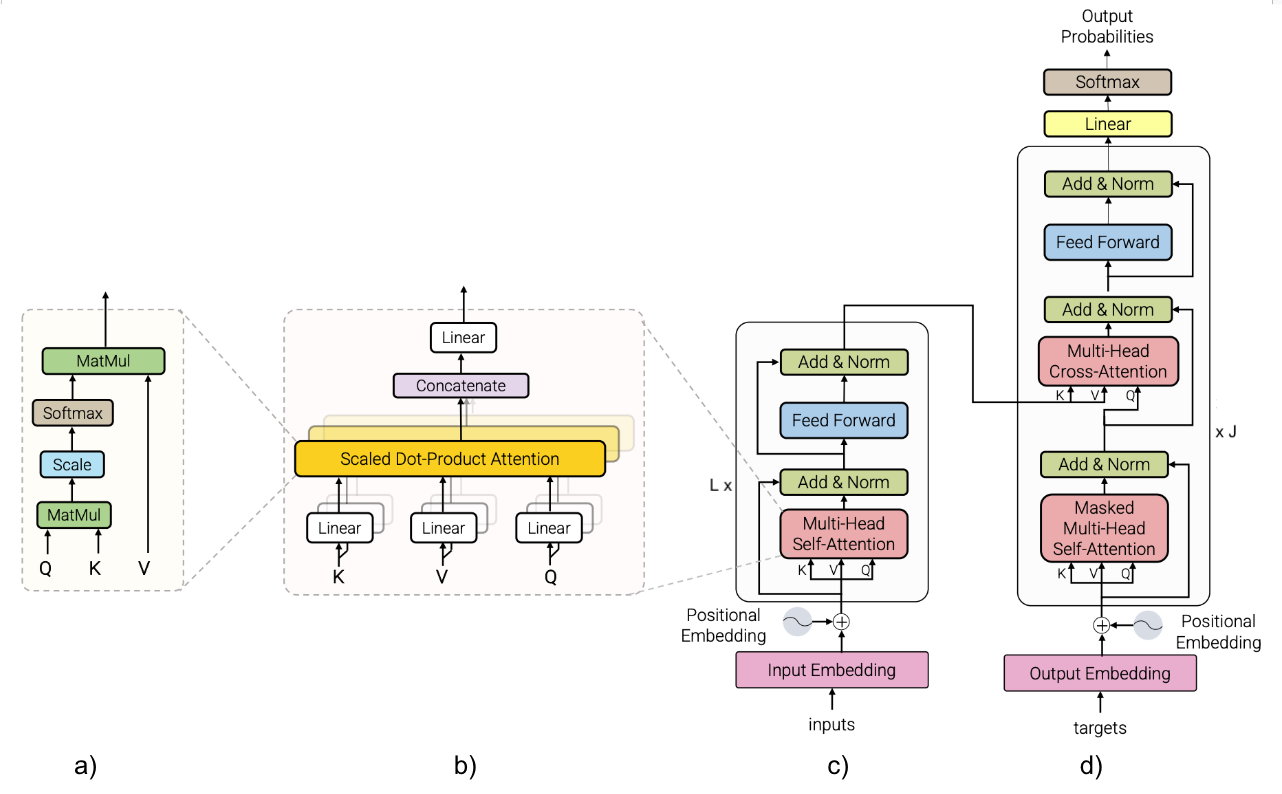
\includegraphics[width=1\textwidth]{imgs/transformer_archi.png}
    \caption{Architecture of the standard Transformer \cite{vaswani2017attention}. a) scaled dot-product attention, b) multi-head self-attention, c) Transformer-encoder, d) Transformer-decoder.}
    \label{fig:transformer_archi}
\end{figure}
% Explain transformer
Introduced in 2017 by Vaswani et al. \cite{vaswani2017attention}, the Transformer architecture is a sequence-to-sequence encoder-decoder model that relies solely on self-attention mechanisms, completely discarding the use of recurrence and convolutions. This design choice addresses challenges such as vanishing gradient issues commonly associated with recurrent neural networks. Another notable difference with recurrent neural networks is that the Transformer computes the dependencies between each pair of positions simultaneously, rather than one by one, by directly encoding the position in the sequence. This enables more parallelisation and therefore a faster training process.

Since its introduction, the Transformer architecture had a tremendous impact across various domains, including Natural Language Processing (NLP) \cite{Bert,brown2020language}, computer vision \cite{dosovitskiy2020image}, and speech processing \cite{dong2018speech}. The Transformer's capacity to capture intricate dependencies and patterns in sequences has established it as a popular architecture in the deep learning field, contributing to advancements and breakthroughs across various applications, such as ChatGPT \cite{bahrini2023chatgpt} or Dall-E \cite{ramesh2021zero}.
%First proposed in 2017 \cite{vaswani2017attention}, the Transformer architecture is a sequence-to-sequence encoder-decoder architecture that relies entirely on self-attention, eliminating recurrence, convolutions entirely and vanishing gradient issues. Another notable difference with recurrent neural networks is that the Transformer computes the dependencies between each pair of positions simultaneously, rather than one by one, by encoding the symbol position in the sequence. This, enables more parallelisation, resulting in faster training. Since its release, the Transformer architecture had tremendous impact in various areas, including NLP \cite{Bert}, computer vision \cite{dosovitskiy2020image}, and speech \cite{dong2018speech}.

The Transformer encoder-decoder architecture, as depicted in Figure \ref{fig:transformer_archi}, consists of an encoder (c) and a decoder (d). Prior to entering the encoder or decoder, both inputs and targets undergo processing through an embedding layer. This involves the use of learned embeddings to convert input tokens and output tokens into vectors of dimension $d_{\text{model}}$. 
% Positional embedding
Since the transformer model contains no recurrence and no convolution mechanisms, information about the relative or absolute position of the tokens must be injected in the sequence to allow the model to make use of the order of the sequence. To achieve this, information about the relative or absolute position of the tokens is obtained through the summation of the input/output embedding and the positional embedding. While various alternatives for positional encodings were used , Vaswani et al. \cite{vaswani2017attention} proposed the use of sinusoidal and cosine functions with different frequencies, as follows:
%Since the transformer model contains no recurrence and no convolution, in order for the model to make use of the order of the sequence, some information about the relative or absolute position of the tokens are injected in the sequence.
%The information about the relative position of the tokens in the sequence is given by the summation between the input/output embedding and the positional embedding. Although there are many choices of positional encodings, \cite{vaswani2017attention} proposed to use sine and cosine of different frequencies as follows:
\begin{align}
    PosEnc_{(pos,2i)} = \sin(pos/10000^{2i/d_{\text{model}}})\\
    PosEnc_{(pos,2i+1)} = \cos(pos/10000^{2i/d_{\text{model}}})
\end{align}
Where $pos$ is the current token or label position and $i$ is the dimension.
 

%Encoder
The encoder's primary objective is to transform the input sequence $X = x_1, \dots, x_T$ into a series of continuous representations $Z = z_1, \dots, z_T$. The encoder is structured as a stack of $L$ identical layers, each comprising two sub-modules: the multi-head self-attention (MHSA) and the position-wise fully connected feed-forward network (FFN). Each of these modules are followed by a normalisation with a residual connection.

%Decoder
Subsequently, the continuous representations $Z$ are fed into the decoder. The decoder is responsible for constructing an output sequence $Y = y_1, \dots, y_N$ one element at a time. At each time step, the decoder receives both the encoder outputs and the last decoder output in an auto-regressive manner. Similar to the encoder, the decoder is composed of a stack of $J$ identical layers. Nevertheless,in comparison to the encoder, the decoder encompasses a third sub-module, which performs multi-head attention (MHA) over the output of the encoder stack. The self-attention sub-module in the decoder stack is modified to prevent positions from attending to subsequent positions. This masking combined with a modified MHA prevents the attention to use subsequent positions, ensuring that the prediction at time-step $i$ solely depends on the previous $< i$ time-steps.


%The transformer encoder-decoder architecture is presented in figure \ref{fig:transformer_archi}, with c) the encoder and d) the decoder. The encoder's role is to transform an input sequence $X = x_1, \dots,x_T$ into a series of continuous representations $Z = z_1, \dots,z_T$ which are then fed into a decoder. The decoder, constructs an output sequence $Y = y_1, \dots, y_N$, one element at a time. At each time step, the decoder receives the encoder outputs together with the last decoder output, in an auto-regressive manner.
% Input embedding



%The encoder is composed of a stack of N identical Transformer layers. Each layer consists of a multi-head self-attention module and a feed-forward fully connected neural network module. Each of these modules are followed by a normalization with a residual connection.
%In comparison to the encoder, the decoder contains a third sub-layer, which performs MHA over the output of the encoder using the prior sub-layer of the decoder as the query. The decoder's inputs, which are targets during training and the previously decoded label during inference, are offset by one position. This combined with a modified MHA prevents the attention to use subsequent positions, ensuring that the prediction at time-step $i$ solely depends on the previous $< i$ time-steps.
%MHSA 
The MHA module relies on scaled dot-product attention \cite{vaswani2017attention}, as illustrated in Figure \ref{fig:transformer_archi}(a). Scaled dot-product attention focuses on determining how relevant a particular token is with respect to other tokens in the sequence and is defined as follows:

\begin{align}
\text{Attention}(Q, K, V) = \text{softmax}\left(\frac{QK^T}{\sqrt{d_k}}\right)V
\label{equation:attention}
\end{align}


Here, the input consists of queries $Q$, keys $K$ of dimension $d_k$, and values $V$ of dimension $d_v$. The dot product of the query with all keys is divided by $\sqrt{d_k}$, and the result passes through a softmax function to obtain attention weights. The attention weights are then multiply with the values. When $d_k$ is large, the scaling  $\frac{1}{\sqrt{d_k}}$ restrains the dot product from growing large in magnitude. Note that the Multi-Head Self-Attention (MHSA) is a specific case of MHA where $K$, $V$, and $Q$ are all the same input of the module.

Instead of performing a single scaled dot-product attention, the MHA module linearly projects $h$ times $K$, $V$, and $Q$ with different, learned, linear projections to dimensions $d_k$, $d_k$, and $d_v$ respectively. The attention function \ref{equation:attention} is then applied in parallel to each of the $h$ projected versions. The output of each of the $h$ attention functions, of dimension $d_v$, is concatenated and projected one final time, as depicted in Figure \ref{fig:transformer_archi}(b). Each of the $h$ attention functions is called a head, while the overall is called Multi-head attention (MHA) or Multi-Head self-attention (MHSA) if $K$, $V$ and $Q$ are the same. More formally:

\begin{align}
\text{MultiHead}(Q, K, V) = \text{Concat}(\text{head}_1, \dots, \text{head}_h)W^O
\end{align}
where
\begin{align}
\text{head}_i = \text{Attention}(QW_i^Q, KW_i^K, VW_i^V)
\end{align}
and the different projection matrices are $W_i^Q \in \mathbb{R}^{d_{\text{model}} \times d_k}$, $W_i^K \in \mathbb{R}^{d_{\text{model}} \times d_k}$, $W_i^V \in \mathbb{R}^{d_{\text{model}} \times d_v}$, and $W^O \in \mathbb{R}^{hd_{v} \times d_{\text{model}}}$.




%A MHA modules relies on the scaled dot-product attention \cite{vaswani2017attention}, illustrated in figure \ref{fig:transformer_archi}.a). Scale dot-product attention focuses on how relevant a particular token is with respect to other tokens in the sequence. And is defined as follows:
%\begin{align}
%    \text{Attention}(Q,K,V) = \text{softmax}(\frac{QK^T}{\sqrt{d_k}})V
%    \label{equation:attention}
%\end{align}
%Where the input consists of queries Q, keys K of dimension $d_k$ and values V of dimension $d_v$. The dot product of the query with all keys is each divided by $\sqrt{d_k}$, then passes through a softmax function to obtain attention weights on the values. When $d_k$ is large, the scaling  $\frac{1}{\sqrt{d_k}}$ restrains the dot product from growing large in magnitude. Note that the MHSA is a particular case of MHA where K,V and Q are all the input of the module.

%Instead of performing a single scaled dot-product attention, the MHA module linearly projects $h$ times K, V and Q with different, learned, linear projections to dimensions $d_k$,$d_k$ and $d_v$ respectively. On each of $h$ projected versions is performed the attention function \ref{equation:attention} in parallel. The output of each of the $h$ attention function, of dimension $d_v$ is concatenated and projected one last time as pictured in figure \ref{fig:transformer_archi}.b). More formally:
%\begin{align}
%    \text{MultiHead}(Q,K,V) = \text{Concat}(\text{head}_1, \dots, \text{head}_h)W^O \\
%    \text{where } head_i = \text{Attention}(QW_i^Q, KW_i^K, VW_i^V)   \nonumber
%\end{align}
%Where the different projections matrices are $W_i^Q \in \mathbb{R}^{d_{\text{model}}\times d_k}$, $W_i^K \in \mathbb{R}^{d_{\text{model}}\times d_k}$, $W_i^V \in \mathbb{R}^{d_{\text{model}}\times d_v}$ and $W^O \in \mathbb{R}^{hd_{v}\times d_{model}}$.


% FFN
Furthermore, in addition to the attention modules, each layer within the encoder and decoder encompasses a FFN module. This network is applied to each position separately and identically, and it consists of two linear transformations with a Rectified Linear Unit (ReLU) activation in between. While attention capture interdependencies between the element of the sequence regardless of their position, the FFN non-linearly transform each input token independently:

\begin{align}
    FFN(x) = max(0,xW_1 + b_1)W_2 + b_2
    \label{equation:FFN}
\end{align}
With $W_1 \in \mathbb{R}^{d_{model} \times d_{ffn}}$, $b_1 \in \mathbb{R}^{d_{ffn}}$, $W_2 \in \mathbb{R}^{d_{ffn} \times d_{model}}$ and $b_2 \in \mathbb{R}^{d_{model}}$. Typically $d_{ffn}$ is usually set to $4 \times d_{model}$.

\section{Conformer model}
\label{sec:conformer}
\begin{figure}[h]
    \centering
    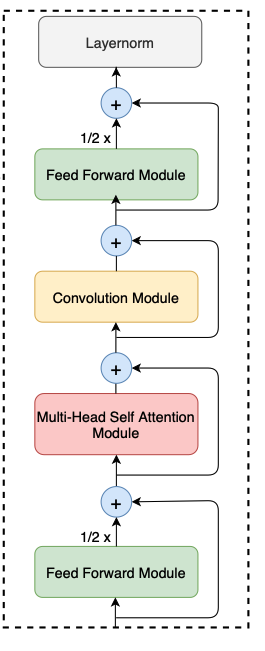
\includegraphics[scale=0.4]{imgs/ConformerLayer.png}
    \caption{Architecture of a Conformer layer}
    \label{fig:conformer_archi}
\end{figure}

\begin{figure}[h]
    \centering
    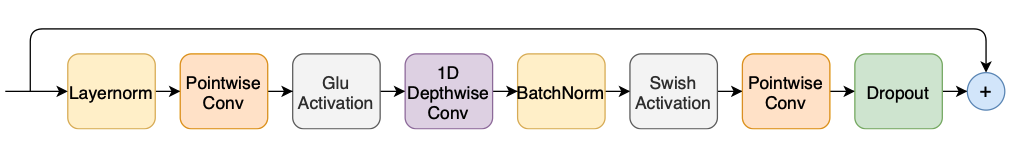
\includegraphics[width=1\textwidth]{imgs/ConvolutionModule.png}
    \caption{Convolution module in the context of a conformer layer}
    \label{fig:convModule}
\end{figure}
Transformers are recognised for their effectiveness in capturing global information within sequential tasks, thanks to the attention mechanism. Conversely, CNNs excel in capturing local features within data. To leverage the complementary strengths of both architectures, various approaches have been explored \cite{bello2019attention,yang2019convolutional}, and the Conformer architecture \cite{gulati2020conformer} stands out as a notable combination of Transformers and CNNs.

This combination involves incorporating CNNs into the conventional Transformer architecture, as depicted in Figure \ref{fig:conformer_archi}. Specifically, a Conformer block comprises four modules arranged sequentially: a FFN module, a MHSA module, a convolution module, and a second FFN module. Notably, the Conformer block features two FFN modules sandwiching the MHSA module and the Convolution module. This design is inspired by Macaron-Net \cite{lu2019understanding}, which advocates replacing the original FFN in the Transformer block with two half-step FFN modules—one before the attention layer and one after. Similar to Macaron-Net, half-step residual weights is employed for the FFN modules. More formally, for an input $x_i$ to a Conformer block $i$, the output $y_i$ of the block is defined as follows:

%While Transformers are known for their effectiveness in capturing global interactions within data, especially in sequential tasks, with the help of the attention mechanism, CNNs excel at capturing local features within data. Consequently, different appraoches tried to use combining Transformer and CNNs, among these the Conformer architecture was introduced to effectively combine the strengths of both Transformers and CNNs. This is achieved by integrating CNNs into the conventional Transformer architecture as shown in figure \ref{fig:conformer_archi}. More specifically, a Conformer block consists of four modules arranged sequentially: a feed-forward module, a self-attention module, a convolution module, and a second feed-forward module. It is important to note that the Conformer block contains two FFN modules sandwiching the MHSA module and the Convolution module, inspired by Macaron-Net, which proposes replacing the original feed-forward layer in the Transformer block into two half-step feed-forward layers, one before the attention layer and one after. As in Macron-Net, we employ half-step residual weights in our feed-forward (FFN) modules.  Mathematically, for input $x_i$ to a Conformer block $i$, the output $y_i$ of the block is:
\begin{align}
    \begin{split}
    \tilde{x_i} = x_i + \frac{1}{2}FFN(x) \\
    x_i^{\prime} =\tilde{x_i} + MHSA(\tilde{x_i}) \\
    x_i^{\prime\prime} = x_i^{\prime} + Conv(x_i^{\prime}) \\
    y_i = LayerNorm(x_i^{\prime\prime} + \frac{1}{2}FFN(x_i^{\prime\prime}))
    \end{split}
\end{align}

More specifically,the convolution modules , inspired by \cite{wu2020lite} and illustrated in Figure \ref{fig:convModule}., starts with a gating mechanism \cite{dauphin2017language} involving a pointwise convolution and a gated linear unit (GLU). Subsequently, a single 1-D depthwise convolution layer is employed. Finally, this 1-D depthwise convolution is followed by a Batchnorm iand then a Swish activation layer.


\section{Understand transfer learning efficacy for transformer based models}
% Explain motivation 
Motivated by the limited availability of children's speech data, TL emerges as a promising strategy to address this challenge in children's ASR. TL involves leveraging pre-trained models, typically trained on extensive datasets of adult speech, and adapting them to the specific characteristics of children's speech through a re-training phase using a smaller, in-domain dataset of children's speech. This approach has demonstrated effectiveness not only in traditional HMM-DNN approaches, as illustrated in the previous chapter \ref{chap:Chapter3} and corroborated by literature \cite{shivakumar2020transfer}, but also in modern end-to-end ASR paradigms \cite{sri_end2end,gelin2021endtoend}.

While the end-to-end paradigm has become state-of-the-art for some children's datasets, particularly when adapted from pre-trained adult models using TL, it involves merging all components of traditional HMM-based ASR pipeline, including acoustic, pronunciation, and language models, into a single neural network. This unique neural network design results in an increased number of parameters. Therefore, there is a need to understand how these large pre-trained models behave when fine-tuned with limited downstream data, as training on a large number of parameters with a small dataset could potentially lead to decreased performances. To address this, we propose a more granular investigation of TL for children's speech using both Transformer and the Conformer architecture.
% Over param of transformer models
Indeed, investigating TL for large-size models is a crucial step in the development of robust children's ASR, given the widely acknowledged issue of overparameterisation in large Transformer-like models. Notably, models like BERT \cite{Bert} have been widely recognised as overparameterised in various studies within the Natural Language Processing (NLP) field \cite{kovaleva-etal-2019-revealing,michel2019sixteen}. Overparameterisation occurs when models have more parameters than necessary for a given task. Observations suggest that certain components or layers of the architecture can be removed without compromising performance, and in some cases, may even lead to slight performance gains \cite{kovaleva-etal-2019-revealing,michel2019sixteen,ye2023partial}. This recognition has fueled successful compression studies, including pruning and distillation techniques \cite{mccarley2019structured,sanh2019distilbert}. 

% Overfitting of large model and loterry ticket hypothesis
Furthermore, the acknowledgment of overparameterisation in Transformer-based models raises questions about the efficiency and computational cost of these architectures. Larger models tend to be more prone to overfitting, as demonstrated in a study where an ASR model was scaled up to 10 billion parameters \cite{zheng22d_interspeech}. Overfitting can be a concern when applying TL as using a overfitted pre-trained model could potentially  leading to decreased performances. Therefore, there is a need for ablation studies, involving the systematic removal of components of the model, to understand which parts contribute significantly to the performances \cite{shen2021partial,wang2021fine}. These studies, predominantly explored in the field of computer vision \cite{ye2023partial}, align with the Lottery Ticket hypothesis formulated by Frankle and Carbin \cite{frankle2018lottery}: 

\begin{quote}
    \textit{``A randomly-initialized, dense neural network contains a subnetwork that is initialized such that—when trained in isolation—it can match the test accuracy of the original network after training for at most the same number of iterations''}.
\end{quote}

Understanding the contribution of the different components of the large-size model not only helps optimise model architectures for specific tasks but also reduces the computational demands of training and inference. This is particularly relevant in scenarios with resource constraints, such as limited computational power, memory, and training data. 


% This work investigate it on children ASR
While these ablation works have been extensively studied in NLP and computer vision, this approach remains under-explored for speech tasks. Specifically, the recent successes of distilation and pruning techniques for speech models \cite{gandhi2023distilwhisper,chang2022distilhubert,peng23c_interspeech}, suggest that overparameterisation is also present in ASR models. In the context of children's ASR, where data scarcity is a significant challenge, understanding and addressing overparameterisation could paves the way for the development of more tailored and efficient models, with improved performances. Notably, the Transformer and Conformer architectures have exhibited promising results in ASR applications, making them particularly compelling subjects for further investigation.


\subsection{Partial Transfer learning}
% Explain experiments

Our aim is to undertake a comprehensive exploration of TL, specifically on end-to-end ASR for children's speech. Notably, previous research in this field has solely been focused on HMM-DNN models, as illustrated by the work of Shivakumar et al. \cite{shivakumar2020transfer}. This previous work provided recommendations for the development of better children's ASR systems, but such a study is currently missing for the end-to-end paradigm, which  further motivated our investigation. It is noteworthy that existing works on the end-to-end paradigm have only centered on the entire model fine-tuning, leaving a notable gap in the understanding of the impact of fine-tuning individual components.

Firstly, we perform a meticulous examination of the TL process, specifically isolating the effects on individual components of the Encoder and Decoder, in comparison to the fine-tuning of the entire model. The prevailing hypothesis asserts that the Encoder is  capturing acoustic information, while the Decoder more linguistic informations. Considering the important presence of acoustic variability in children's speech, our investigation extended to discern which layers of the Encoder are more relevant for achieving effective TL.

Subsequently, our focus shifts to delineating the distinctive contributions of modules within both the Transformer and Conformer architectures during the fine-tuning process of adapting a pre-trained adult model to children's speech. Within the Transformer model, a granular analysis will be conducted to asses the roles of the MHSA module, the FFN, and the normalisation layers independently. Similarly, within the Conformer model, we evaluate the significance of the MHSA, FFN, normalisation, and convolution modules. This exhaustive examination is meticulously designed to identify the components that play a pivotal role in fine-tuning.


\subsection{Experimental setup}
\label{section:methods_chapter4}

\subsection{Corpus}
\begin{table}[ht]
\centering
\begin{tabular}{c|c|c}
\hline
 Training & Validation     & Test   \\ \hline
60897 utterances  & 10044 utterances   & 4079 utterances \\ 
 566 speakers  & 79 speakers   & 91 speakers \\ 
 113 hours  & 18 hours   & 13 hours \\ \hline

\end{tabular}
\caption{My Science Tutor Children Speech Corpus statistics}
\label{tab:statistics_myst}
\end{table}
In this experiment, we decided to used  the Boulder Learning My Science Tutor (MyST) corpus, as detailed in section \ref{section:children_corpora}. This choice aligns with the nature of the task assigned to the children in the MyST corpus, which involves spontaneous speech. The the end-to-end paradigm, by encapsulating both the acoustic model and language model within the same network, requires careful consideration. Indeed, if the model is trained on a limited set of prompts, from a dataset focused on reading tasks for example, it may learn and overfit to those specific prompts, yielding unreliable results.

For the purposes of our experiments, we decided to remove all utterances shorter than one second and longer than 20 seconds and shorter than one second. Typically, utterances shorter than one second were found to predominantly contain silence alone, while those longer than 20 seconds were constrained by our GPU limitations. The details of the filtered corpora used in our work are presented in Table \ref{tab:statistics_myst}. 

%In this work, we decided to use the Boulder Learning My Science Tutor (MyST) corpus, described in section \ref{section:children_corpora} given the task assigned to the children, which is to speak spontaneously. Indeed, the end-to-end model encapsulates the acoustic model and language model in the same network. As a result, if we train a model with a restricted amount of prompts on a data set of reading tasks, the model will learn and overfit the prompts. Thus, yielding unreliable results. Furthermore, for the purposes of our experiments, we decided to remove all utterances shorter than one second and longer than 20 seconds. The details of the filtered corpora used in our work are presented in Table \ref{tab:statistics_myst}. 
\subsection{Implementation details}

% Transformer  and Conformer model description
All experiments were conducted using the SpeechBrain toolkit \cite{speechbrain}. The Transformer model encompasses 12 Transformer layers in the encoder and 6 Transformer layers in the decoder, all with a hidden dimension of 512. Similarly, the Conformer architecture featured 12 Conformer layers in the encoder and 6 Transformer layers in the decoder, with a hidden dimension of 512. Both configurations used 8 heads for all MHSA, a FFN hidden dimension of 2048, and a dropout rate of 0.1. These models were pre-trained on a large English adult speech corpus, specifically the LibriSpeech dataset \cite{librispeech}, and are publicly available\footnote{https://huggingface.co/speechbrain/asr-transformer-transformerlm-librispeech\\ https://huggingface.co/speechbrain/asr-conformer-transformerlm-librispeech}. Furthermore, for all experiments, the same Transformer language model was employed, trained on 10 million words from LibriSpeech transcriptions. Our training involved 30 epochs with a learning rate of 8e-5. Furhtermore, in line with findings of \cite{gelin2021endtoend}, a combination of CTC and Seq2Seq losses was used, with respective weights of 0.3 and 0.7.

% TODO Should the url being citation with "last check on XX/12/23"?

\subsection{Encoder-Decoder Transfer learning}
% Encoder - Decoder
\begin{table}
    \begin{center}
        \begin{tabular}{lcc}\hline
            Transformer    &   WER $\downarrow$    & Trained parameters  \\ \hline
            Full model          & 12.99\% & 71.5M   \\
            Encoder only & \textbf{12.55\%} & 37.8M  \\
            Decoder only & 15.95\% & 25.2M  \\ \hline \hline
            Conformer    &    & \\ \hline
            Full model          & 12.28\% & 109M   \\
            Encoder only & \textbf{11.24\%} & 75.9M  \\
            Decoder only & 16.94\% & 25.2M  \\ \hline 

        \end{tabular}
    \end{center}
    \caption{Encoder-Decoder experiment}
    \label{tab:EncoderDecoder}
\end{table}
Table \ref{tab:EncoderDecoder} summarises the results of the impact of isolating fine-tuning of the encoder and decoder components within Transformer and Conformer ASR models. For the Transformer model, using fine-tuning then entire model exhibits a WER of 12.99\% using 71.5 million parameters. Isolating the encoder component leads to a significant improvement in WER, with TODO\% WER with a reduced parameter count of 37.8 million. Parallely, fine-tuning the decoder underperform compared to both full model and Encoder only fine-tuning by achieving a WER score of 15.95\% training 25.2 million parameters. 

Turning to the Conformer model, the full model achieves a WER of 12.28\% with 109 million parameters updated. Isolating the transfer learning on the encoder component only  yields a remarkable improvement, resulting in a WER of 11.24\% with a parameter count of 75.9 million. Conversely, when the decoder only is fine-tuned the performances degrade with a higher WER of 16.94\% using a parameter count of 25.2 million. Notably, the Conformer architecture consistently outperform the Transformer across all configurations, emphasising its effectiveness for speech related tasks. In addition, these results underscore the important role of the encoder in both Transformer and Conformer ASR models, highlighting its importance in capturing the inherent variabilities in children's acoustics. It confirms that the acoustics variabilities represent the most important source of variabilities as suggested by \cite{TFchildren}.

% Layers wise
\begin{figure}
    \centering
    \subfigure[Results of the transfer learning layer wise for the Transformer model]{\label{fig:transferTLTransformer}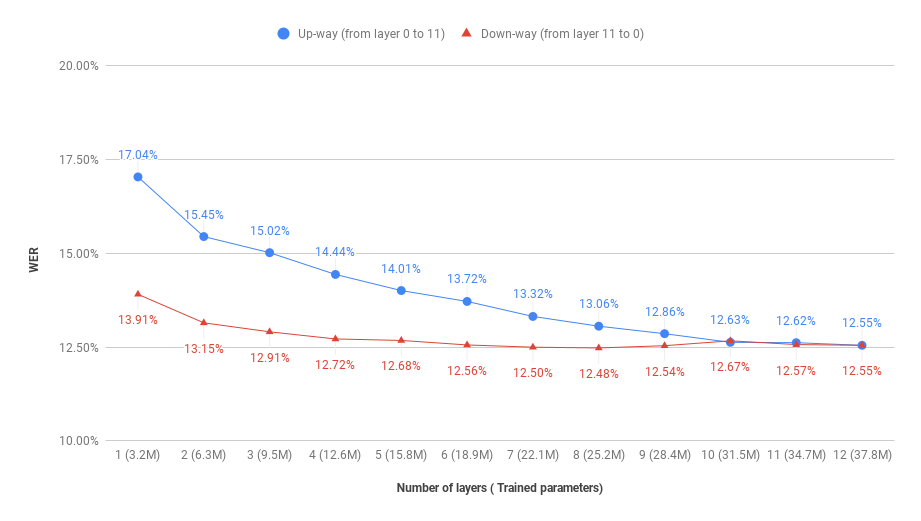
\includegraphics[width=0.7\textwidth]{imgs/layerTL_transformer.png}}
    \subfigure[Results of the transfer learning layer wise for the Conformer model]{\label{fig:transferTLConformer}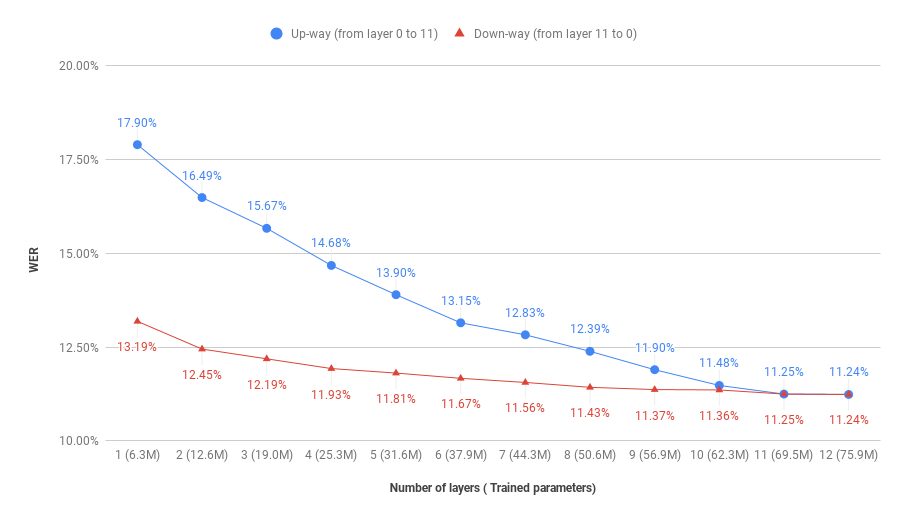
\includegraphics[width=0.7\textwidth]{imgs/layerTL_conformer.png}}
    \caption{Layers-wise up-way and down-way transfer learning experiment for Transformer and Conformer architecture}
    \label{fig:layerWISE}
\end{figure}

%\begin{figure}
%    \begin{center}
%        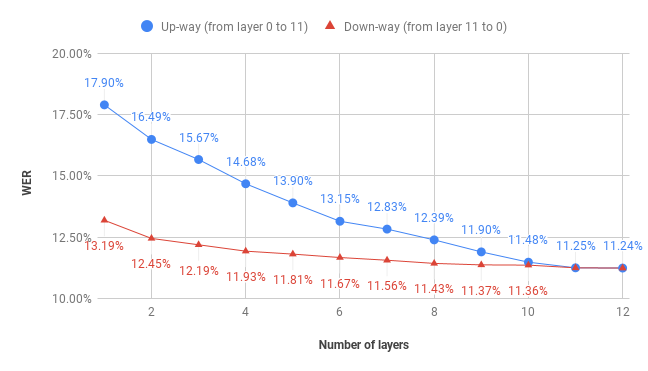
\includegraphics[scale=0.7]{imgs/layerTL.png}
%    \end{center}
%    \caption{Up-way and down-way transfer learning experiment}
%\end{figure}
Recognising the pivotal role of the Encoder in the success of the fine-tuning process for children's ASR, our investigation delves deeper to determine the specific layers that are the most important during this TL process. To this end, we adopt a meticulous approach where we incrementally fine-tuned the Encoder by adding one layer at a time for each fine-tuning experiment. This layer-wise fine-tuning procedure is executed bidirectionally, encompassing both an up-ward trajectory, commencing from the input layer, and a down-ward trajectory, starting from the output layer of the Encoder. In other words, the up-ward trajectory involves progressively fine-tuning by adding one layer at a time for each experiment, starting from the input layer and systematically integrating subsequent layers towards the output layer of the Encoder. Conversely, the down-ward trajectory initiates fine-tuning from the output layer, systematically incorporating preceding layers towards the input layer at each experiments. The results of this layer-wise fine-tuning procedure for both the Transformer and Conformer architectures are presented in Figure \ref{fig:layerWISE}.

In both the Transformer and Conformer scenarios, a consistent pattern emerged. The incremental addition of more layers was found to be consistently beneficial, with optimal performance stabilisation occurring when 10 layers out of the 12 are employed. we observed the advantage of utilising TL from the top layers in the down-ward direction (i.e., those close to the output of the Encoder) compared to the bottom layers in the up-ward direction (i.e., those close to the input of the Encoder). The success of the up-ward trajectory, in contrast to the down-ward trajectory, indicates that the top layers of the Encoder are the most relevant for fine-tuning in the context of children's speech. This exploration of layer-wise fine-tuning sheds light on the intricate dynamics of TL within the Encoder, offering valuable insights into the targeted layers that significantly contribute to optimising the performance of children's ASR models. 
%Recognising the important role of the Encoder in the fine-tuning process for children ASR, our investigation further look to determine the specific layers that are the most relevant during this TL process. To this end, we adopt a meticulous approach of fine-tuning the Encoder incrementally, adding one more layer for each experiment. This incremental TL procedure is executed in each directionally, one commencing from the input layer while the other one from the output layer of the encoder,the up-way and down-way respectively. In other words, the up-way, for each experiments we incrementally fine-tuning by adding one layere a the time. Begining with the input layer and progressively incorporating subsequent layers towards the output layer. While, the down-way initiates fine-tuning from the output layer, systematically integrating preceding layers towards the input layer at each experiment. We present the results of this layer-wise fine-tuning for both Transformer and Conformer in Figure \ref{fig:layerWISE}.
%In both the Transformer adn Conformer scenario, we observed a similar behavior. Adding more layers was found always beneficial, with a stabilisation of the best performances when 10 layers out of the 12  are used to fine-tuned the model. An interesting observation, was the fact that using transfer learning from the top layers (i.e. close to the output of the Encoder) was found more beneficial than from using transfer learning from the bottom layers (i.e. close to the input of the Encoder). The success of the Up-way compared to the Down-way indicates that the top layers of the Encoder are the most relevant to fine-tune in the context of Children's speech.
\subsection{Modules Transfer learning}
% Block wise
\begin{table}
    \begin{center}
        \begin{tabular}{lcc}\hline
            \textbf{Transformer}    & WER  $\downarrow$   & Trained parameters \\ \hline
            None & 25.04\% & -   \\
            Full model   & 12.99\% & 71.5M   \\ \hline
            Normalisation & 17.00\% & 57.9K  \\
            MHSA & 12.19\% & 25.2M  \\
            FFN    & \textbf{11.84\%}     &  37.8M \\ \hline
            MHSA + FFN & 12.39\% & 63.0M \\
            Normalisation + FFN & 12.19\% & 37.9M \\
            Normalisation + MHSA & 12.29\% & 25.3M\\ \hline \hline
            \textbf{Conformer}    &     & \\ \hline
            None & 21.75\% & -   \\
            Full model   & 12.28\% & 109M   \\ \hline
            Normalisation & 15.61\% & 63.7K  \\
            MHSA & 11.74\% & 28.4M  \\
            Convolution Module & 11.67\% & 9.7M \\
            FFN    & \textbf{11.10\%}     &  63M \\
            \quad $\hookrightarrow$ Module 1    & 11.44\%     &  25.2M \\
            \quad $\hookrightarrow$ Module 2    & 11.48\%     &  25.2M \\
            \quad $\hookrightarrow$ Up-linear ($W_1$)    & 11.47\%     &  31.5M \\
            \quad $\hookrightarrow$ Down-linear ($W_2$)    & 11.40\%     &  31.5M \\ \hline
            FFN + MHSA & 11.20\% & 91.4M \\
            FFN + Convolution Module & 11.11\% & 72.7M \\
            FFN + Normalisation & 11.15\% & 63.1M \\
            MHSA + Normalisation & 11.67\% & 28.4M \\
            MHSA + Convolution Module & 11.44\% & 38.0M \\
            Convolution Module + Normalisation & 11.62\% & 9.7M\\ \hline
        \end{tabular}
    \end{center}
    \caption{Modules fine-tuning experiment}
    \label{table:ModulesTL}
\end{table}
The results  of the transfer learning experiments, focusing on fine-tuning specific components of the Transformer and Conformer ASR models for children's speech, are presented in Table \ref{table:ModulesTL}. In addition of the WER evaluation metric, we also display the number of trained parameters. 

% Transformer
The baseline performance of the Transformer pre-trained model without any fine-tuning (corresponding to \textit{None} line) yields a WER of 25.04\%. In contrast, the fine-tuning of the full Transformer model exhibits a noteworthy improvement, achieving a WER of 12.99\% with 71.5 million parameters trained.

The fine-tuning of specific components reveals valuable observations. Applying normalisation alone results in a modest improvement WER of 17.00\% compared to keeping the pre-trained model, this using 57.9 thousand parameters. The MHSA module outperforms normalisation and full fine-tuning, achieving a WER of 12.19\% with a parameter count of 25.2 million. However, the most important improvement is observed with the FFN module, which attains a remarkable WER of 11.84\% with 37.8 million parameters. Remarkably, both MHSA and the FFN modules, when fine-tuned individually, already outperform the full model performance. This implies that the decrease in the number of parameters, coupled with the significance of these modules, may play a substantial role in the enhanced performances.

%Conformer
Turning to the Conformer model, the baseline WER without fine-tuning is 21.75\%, with no additional parameters. The full fine-tuning of the Conformer model improved performance, yielding a WER of 12.28\% with 109 million parameters.

Fine-tuning specific Conformer modules offers further granularity. First, the normalisation finetuning, in a similar way as observed in the Transformer configuration, yield a score of 15.61\% WER, with 63.7 thousand parameters. Then,  the MHSA module proves effective by already providing better result than the full full-tuning with a WER of 11.74\%, this by fine-tuning 28.4 million parameters. The convolution modules outperform the MHSA with a WER of 11.67\% with less parameters used, 9.7\%. Howver, as in the Transformer model, the FFN module stands out prominently, demonstrating a WER of 11.10\% with a parameter count of 63 million. Notably, the MHSA, convolution modules and FFN modules, when fine-tuned in isolation, surpass the performance of the full Conformer model.

% FFN wise
As FFN, consistently proved to be the most relevant component to fine-tune for children ASR, no matter the configuration. We decided to delve deeper into the FFN submodule. There is two way to see this subdivision, first using the macaron style of the Conformer FFn layer, including two modules, one before the MHSA and one after the convolution module will be respectively called Module 1 and Module 2. The second approach to subdivde the FFN layers would be to only look at the up-linear and down-linear, respectively $W_1$ and $W_2$ equation \ref{equation:FFN}. Module 1 and Module 2 achieve WERs of 11.44\% and 11.48\%, respectively, each by fine-tuning 25.2 million parameters. The Up-linear and Down-linear  submodules exhibit WERs of 11.47\% and 11.40\%, respectively, with parameter counts of 31.5 million. The subdivision of the FFN modules do not allow to perform better than their coupled usage. This show the importance of the full FFN modules in Transformer based end-to-end models. 

%Combination of different components
Furthermore, our investigation delved into the impact of combining different components within both the Transformer and Conformer architectures. In the case of the Transformer model, the results consistently demonstrated that while all combinations improved the 12.99\% WER achieved through full model fine-tuning, they consistently underperformed the score of the FFN component alone of 11.84\% WER. The most promising combination attained a WER score of 12.19\%, by using the Normalisation and the FFN in combination.
Similarly, within the Conformer architecture, a comparable trend emerged. While all combinations exhibited improvements compared to full model fine-tuning score of 12.28\%, they still lagged behind the performance achieved with the FFN-only scenario of 11.10\%. A noteworthy result was the observation that the combination of the FFN and convolution modules proved to be as effective as the FFN in isolation, yielding a WER score of 11.11\%. This particular experiment accentuates the notion that employing a single component is more advantageous than utilising combinations, thereby suggesting the merits of a more parsimonious use of parameters.

This observation aligns with the concept of the Lottery Ticket Hypothesis, which posits that within a neural network, there exist subnetworks (winning tickets) that, when isolated, can perform equally well as the full network. In the context of transfer learning for children's end-to-end ASR, the findings underscore the effectiveness of a focused and selective utilisation of components, reflecting a nuanced and strategic approach to optimising model performance.

\section{Summary and discussion}

% Research question
In this chapter, we delve into the end-to-end paradigm for children's ASR, particularly using transfer learning from a pre-trained adult model. We aimed to answer the following research questions: \textit{How do end-to-end automatic speech recognition models achieve state-of-the-art results for children's ASR when finetuned from an adult model? Particularly, what are the components that are most important to fine-tune?}

In contrast to prior research where fine-tuning involved the entire network, our detailed evaluation of different level of fine-tuning provides insights into the underlying behavior of the model when adapted to children's ASR. This research offers valuable recommendations for the future development of children's end-to-end ASR systems. Initially, we identified the Encoder as the most crucial part of the model to fine-tune compared to the Decoder. This aligns with the hypothesis that the substantial variability in children's speech is present in the acoustics and can be effectively captured in the Encoder, echoing similar findings in transfer learning experiments for HMM-DNN framework \cite{TFchildren}.

Addressing the second research question, our proposed partial fine-tuning procedure sheds the light on the most important components for adaptation in both Transformer and Conformer architectures. This experiment unveiled the presence of the Lottery Ticket Hypothesis in such end-to-end architectures, indicating over-parameterization. Through our partial fine-tuning approach, the FFN module emerged as the most critical component to fine-tune, outperforming all other configurations, even the entire model fine-tuning. Previous research \cite{geva2020transformer} has revealed that FFN layers exhibit key-value memory properties, offering a plausible explanation for their success in the transfer learning procedure. Moreover, we observed that combining these submodules can potentially deteriorate ASR results, underscoring the challenge of over-parameterisation and the need of training on smaller amount of parameters. This emphasises the effectiveness of our granular partial fine-tuning process for end-to-end models with small datasets.

% Discussion
As the ASR field advances, one notable trend is the ever-increasing size of models, where parameters in neural networks are reaching unprecedented scales. Within these expansive architectures, the FFN often constitute a substantial portion of the model's overall parameter count. The FFN component, responsible for processing and transforming information through hidden layers, contributes significantly to the model's complexity.

The widespread adoption of massive models has raised concerns regarding computational efficiency, optimal resource utilisation, and the potential risk of overfitting when these models are fine-tuned with limited data. Given that FFNs modules constitute a substantial portion of these large-scale models, there is an gained interest in developing parameter-efficient transfer learning strategies. Efficient utilisation of parameters during training is not only crucial for mitigating computational costs but also for enhancing the practicality of deploying these models in real-world scenarios where limited resources may exist.
The next chapter of this thesis will delve into the feasibility of employing such parameter-efficient approaches for children's ASR. Such parameter-efficient approach could be highly beneficial in the context of speaker-based ASR systems for children. 

%We covered the state-of-the-art for end-to-end children's speech recognition in this chapter. Particularly, the usage of the Transformer architecture in conjunction with transfer learning. In a similar way as chapter \ref{chap:Chapter3}, to avoid a drop in performances attributable to an acoustic mismatch between children and adults, the end-to-end model should be trained with children's data. In contrast to previous work, we demonstrated that fine-tuning only a portion of the transformer modules, particularly the FFN sub-module, yields better results since it serves as a key-value memory. As a result, we placed our adapter subsequent to it. The adapter's role is to accomplish knowledge transfer, which is related to transfer learning. Rather than updating the complete model's weights, we just tweak an extra module, hence fewer parameters. This adapter transfer achieves almost identical results as the entire model fine-tuning. In addition, adapters are useful in the context of customized models, where training and storing a whole model for each age group or each child can be expensive and time-consuming.

%In addition, we proposed the variational adapter, a variant of the traditional adapter based on variational auto-encoders. Compared to the adapter, which takes a bottleneck encoder-decoder structure with a linear layer as encoder and a linear layer as decoder, the variational adapter's encoder consists of two branches, $\mu$ and $\sigma$. The outputs of these two branches are used as the mean and variance vector to sample the input of the decoder. By doing so, we enforce the adapter's input variability to be contained in the $\sigma$ branch. A branch which is suppressed during inference. As a result, we reduce input variability while maintaining the same size as standard adapters.